%
% teil3.tex -- Beispiel-File für Teil 3
%
% (c) 2020 Prof Dr Andreas Müller, Hochschule Rapperswil
%
\section{Der Munkres-Algorithmus (Ungarische Methode)
\label{munkres:section:teil3}}
\rhead{Der Munkres-Algorithmus (Ungarische Methode)}

Mit der ungarischen Methode können also Optimierungsprobleme gelöst
werden, die bei gewichteten Zuordnungen in bipartiten Graphen entstehen.
Mit ihr kann die eindeutige Zuordnung von Objekten aus zwei Gruppen so
optimiert werden, dass die Gesamtkosten minimiert werden bzw.~der
Gesamtgewinn maximiert werden kann.

\subsection{Geschichte
\label{munkres:subsection:malorum}}
Die Ungarische Methode wurde 1955 von Harold Kuhn entwickelt und veröffentlicht.
Der Name ``Ungarische Methode'' ergab sich, weil der Algorithmus
weitestgehend auf den früheren Arbeiten zweier ungarischer Mathematiker
basierte: Dénes Kőnig und Jenő Egerváry.
James Munkres überprüfte den Algorithmus im Jahr 1957 und stellte fest,
dass der Algorithmus (stark) polynomiell ist.
Seitdem ist der Algorithmus auch als Kuhn-Munkres oder
Munkres-Zuordnungsalgorithmus bekannt.
Die Zeitkomplexität des ursprünglichen Algorithmus war $O(n^4)$,
später wurde zudem festgestellt, dass er modifiziert werden kann,
um eine  $O(n^3)$-Laufzeit zu erreichen.

\subsection{Besondere Leistung der Ungarischen Methode
\label{munkres:subsection:malorum}}
Die Ungarische Methode ist ein kombinatorischer Optimierungsalgorithmus, der das Zuordnungsproblem
in polynomieller Zeit löst.
Der Begriff polynomielle Laufzeit bedeutet, dass die Laufzeit des Programms
wie $n^2$, $n^3$, $n^4$, etc.~wächst und vernünftig skaliert. $n$ ist hierbei die ''Grösse'' des Problems.

\subsection{Unterschiedliche Anzahl von Quellen und Zielen
\label{munkres:subsection:malorum}}
Es gibt Fälle, in welchen das Ausgangsproblem keine quadratische Form besitzt. Das ist z. B. dann der Fall, wenn drei Mitarbeiter vier verschiedene Eignungstests absolvieren müssen. In diesem Fall wird in der Ungarischen Methode die Matrix künstlich mittels einer Dummy Position zu einem Quadrat ergänzt. Dummy-Positionen werden dann mit der größten vorhandenen Zahl aus der Matrix besetzt. Beispielsweise wird eine $3\times 4$ zu einer $4\times 4$-Matrix.

\subsection{Beispiel eines händischen Verfahrens
\label{munkres:subsection:malorum}}

Die ungarische Methode kann in einem einfachen händischen Beispiel erläutert werden. Wir gehen von der Kostenmatrix $A$ aus. Diese Matrix wird in mehreren Schritten immer weiter reduziert. Anschliessend erfolgen mehrere Zuordnungen. Hierbei ist zu beachten, dass jede Zeile und jede Spalte immer genau eine eindeutige Zuordnung ergibt. Es gibt Situationen, in denen man nichts mehr tun muss, um eine optimale Zuordnung zu finden. Eine optimale Zuordnung ohne zusätzliche Kosten ist eine Auswahl genau eines Feldes in jeder Zeile und Spalte, welches 0 enthält. Das Ziel des Algorithmus ist also, die Matrix so zu ändern, dass genügend Nullen in der Matrix vorkommen. Es ist zudem wichtig, dass man nach jeder Modifikation der Matrix testet, ob man bereits eine Zuordnung machen kann, also genügend Nullen hat.
Das Vorgehen wird in den nachfolgenden Schritten 1-6 beschrieben und auch in der Abbildung 21.5 dargestellt.

\begin{enumerate}
\item Man beginnt mit der Zeilen-Reduktion. Pro Zeile eruiert man die kleinste Zahl. Diese kleinste Zahl, jeweils in rot markiert, wird bei allen anderen Ziffern in der jeweiligen Zeile subtrahiert. Mit dieser Subtraktion zieht man die unvermeidbaren Kosten ab, die man hat, um eine Baustelle zu erreichen. Man erkennt, dass die Nullen mit zwei Linien abdeckbar sind. Das heisst es gibt zwei Spalten bei denen noch keine Zuordnungen möglich sind. 

\item Auch im zweiten Schritt werden mittels der Spalten-Reduktion die unvermeidbaren Weg-Kosten abgezogen. Man zieht die kleinste Zahl, wiederum in rot markiert, in jeder Spalte von allen Zahlen in der Spalte ab.
Die Nullen können somit mit drei Linien abgedeckt werden. Im Idealfall hat die Matrix in jeder Zeile und Spalte bereits genügend viele Nullen, so dass man bereits eine Zuordnung ohne Mehrkosten machen kann. Dies ist jedoch noch nicht der Fall. Es sollen weitere Nullen in die Matrix hineingebracht werden.

\item Es bleiben jetzt einige Felder übrig, für die noch keine Zuordnung möglich ist. Die kleinste Ziffer wird dabei aus den noch nicht mit blau markierten Zahlen ausgewählt werden. Im Beispiel ist es die Zahl 1. Das Feld mit dem kleinsten Eintrag beinhaltet die Kosten, die unvermeidlich sind, wenn man für diese Felder auch noch eine Zuordnung machen will. Um neue Nullen zu bekommen, lagert man jetzt die Kosten auf die anderen Zeilen und Spalten um. Dies tut man, indem man in allen nicht abgedeckten Feldern die minimalen Kosten subtrahiert und in den blau markierten Kreuzungspunkten dazu addiert.
Dieser Schritt 3 muss so oft wiederholt werden, bis genügend viele Nullen in der Matrix vorhanden sind.

\item In Schritt 4 sollen jetzt möglichst viele Nullen markiert werden, welche freistehend sind.
Freistehend bedeutet, dass sowohl in der jeweiligen Zeile und Spalte keine andere markierte Null vorhanden ist.

\item Alle markierten Nullen werden jetzt in eine 1 umgewandelt. Die restlichen Ziffern in der Matrix, exklusiv die einsen, sollen jetzt ignoriert und durch eine Null ersetzt werden.

\item Zu guter Letzt werden überall wo eine 1 steht, die Zahlen aus der Ausgangsmatrix eingefügt. Nach Einsetzen der Zahlen können die in rot markierten Zahlen aufsummiert werden. Man erhält den minimalsten Transportweg von total 13 Kilometer.
\end{enumerate}

\begin{figure}
\centering
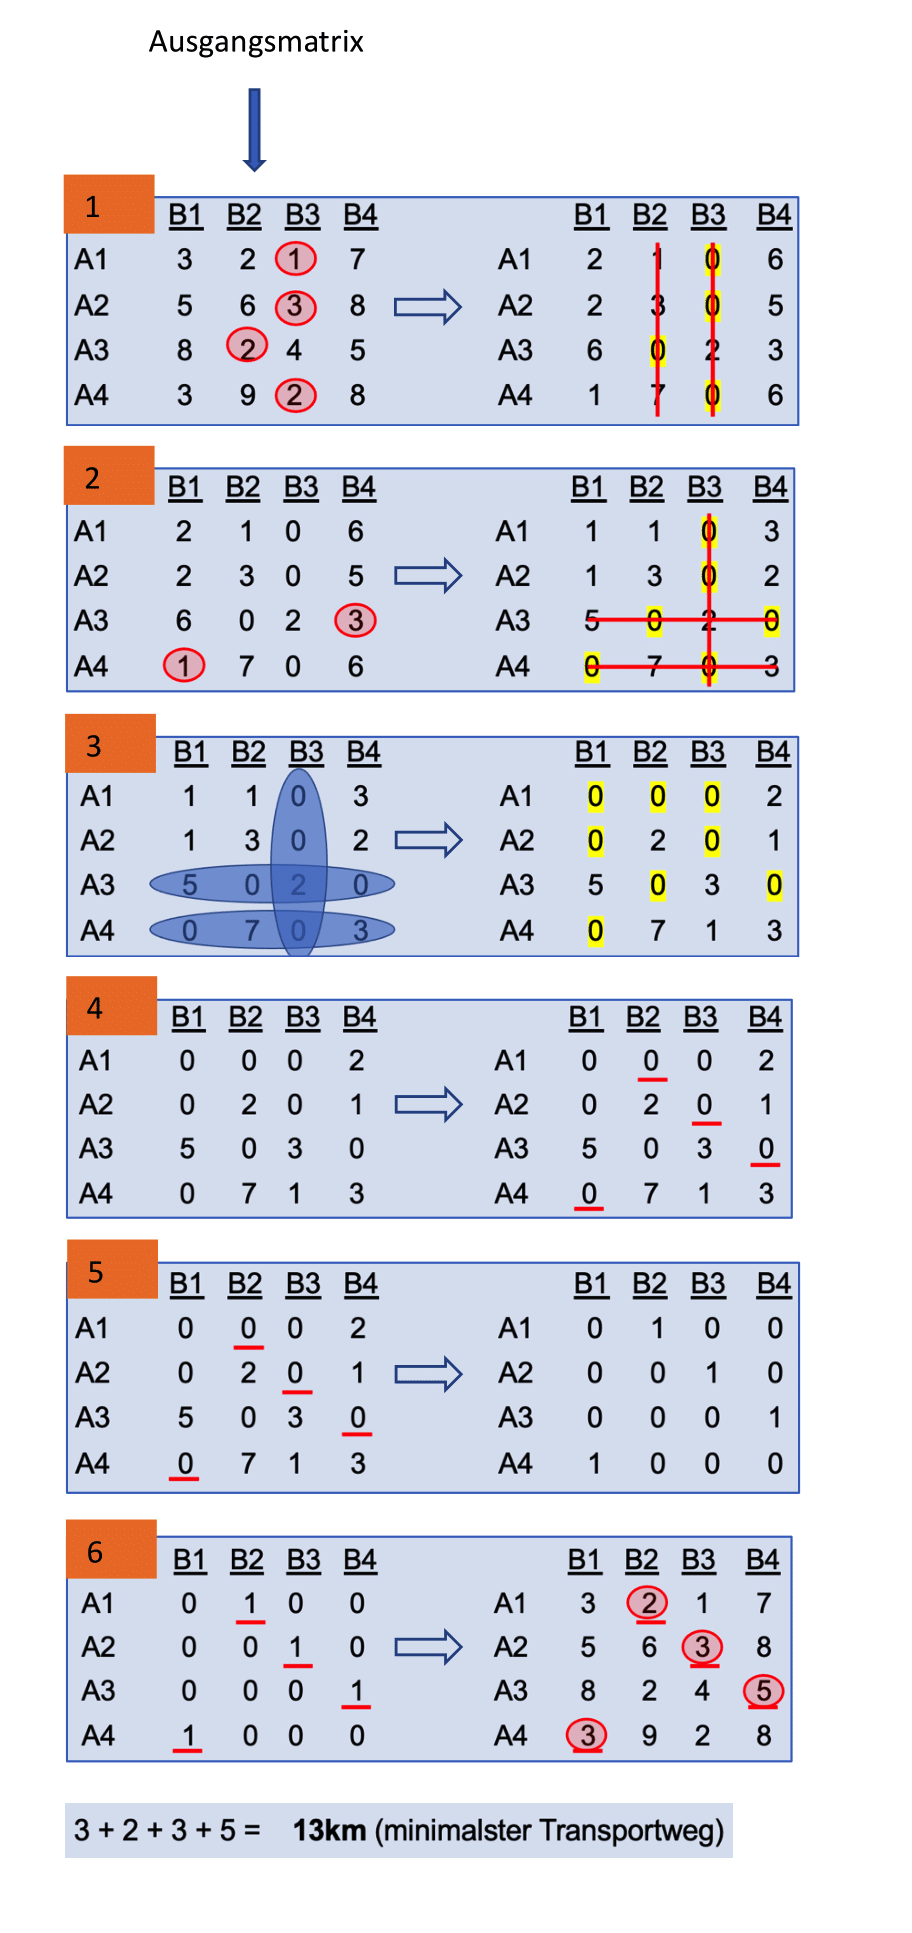
\includegraphics[width=8cm]{papers/munkres/figures/Ungarische_Methode_Beispiel.png}
\caption{Händisches Beispiel des Munkres Algorithmus, minimalster Transportweg.}
\label{munkres:Vr2}
\end{figure}

\subsection{Zuordnung der Kräne
\label{munkres:subsection:malorum}}

Als Resultat des Munkres-Algorithmus werden in Abbildung 21.6 nebst dem minimalsten Transportweg auch die optimalste Zuweisung der Kräne auf die neuen Standorte ersichtlich.
Es können die folgenden Zuordnungen aus der Matrix abgelesen werden:
\begin{itemize}
\item Der Kran von Baustelle A1 soll zur Baustelle B2.
\item Der Kran von Baustelle A2 soll zur Baustelle B3.
\item Der Kran von Baustelle A3 soll zur Baustelle B4.
\item Der Kran von Baustelle A4 soll zur Baustelle B1.
\end{itemize}

\begin{figure}
\centering
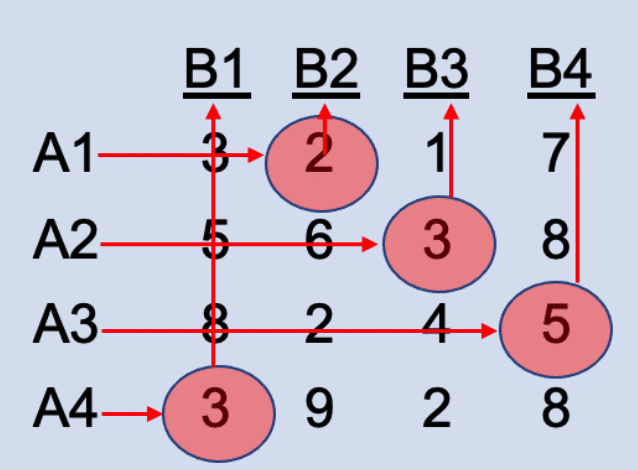
\includegraphics[width=3cm]{papers/munkres/figures/Ungarische_Methode_Beispiel_Zuw.png}
\caption{Händisches Beispiel des Munkres Algorithmus, Zuweisung der Kräne }
\label{munkres:Vr2}
\end{figure} 